\section{Introduction}


In Chapter \ref{ch:ReactionModels} we have established that our "Symmetric" and "Asymmetric" HDAC6 complex formation models are capable of predicting capsid breakage in normal and perturbed conditions. Our next point of interest is to try and use them to make predictions for cases for which we don't know the answer for.

One possible application has been suggested by the data provided by our collaborators from Patrick Matthias' group at FMI. They used designed ankyrin repeat proteins (DARPins) - artificial proteins which can bind target proteins with high affinity and specificity - to try and find one capable of inhibiting HDAC6-mediated influenza uncoating.

\begin{figure}
\begin{center}
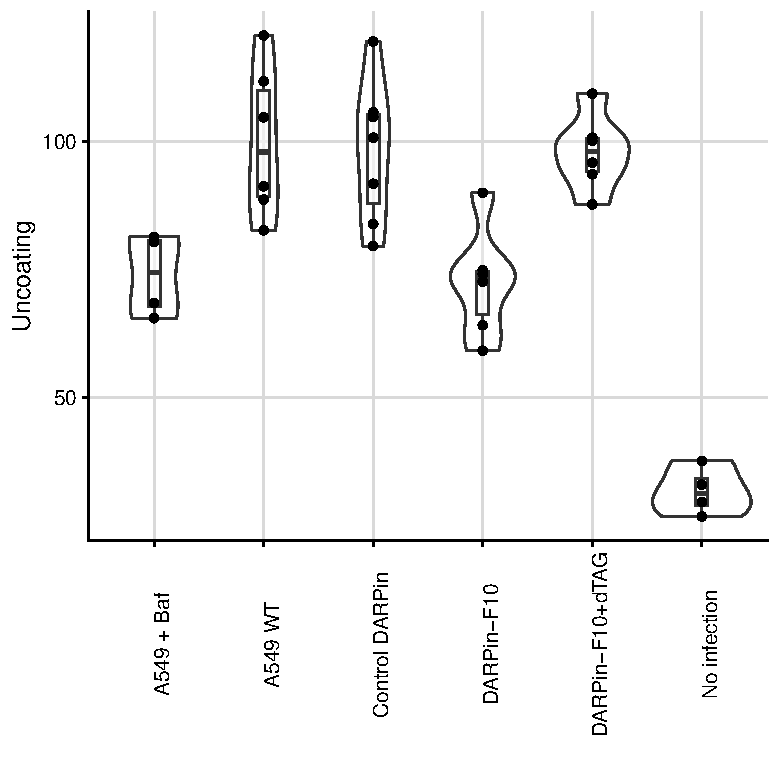
\includegraphics[width=0.95\textwidth, trim={0cm 0cm 0cm 0cm}, clip]{D_chapters/3_DARPinModels/DarpinUncoating.pdf}
\caption[DARPin F10 reduces influenza virus uncoating]%
{DARPin F10 at MOI = 30 PFU/ml reduces influenza virus uncoating\par
A549 + Baf: the cells treated with Bafilomycin, an ATPase inhibitor which also stops viral uncoating;\par
A549 WT: wild type;\par
CTR DARPin: cells with a DARPin that did not bind anything;\par
DARPin-F10: cells with a DARPin that binds HDAC6 ZnF;\par
DARPin-F10 + dTAG: cells in which DARPin F10 was degraded through dTAG before virus infection;\par
* No infection: cells without any virus added to them.}
\label{figure:darpinUncoatingExperimental}
\end{center}
\end{figure}

\begin{figure}
\begin{center}
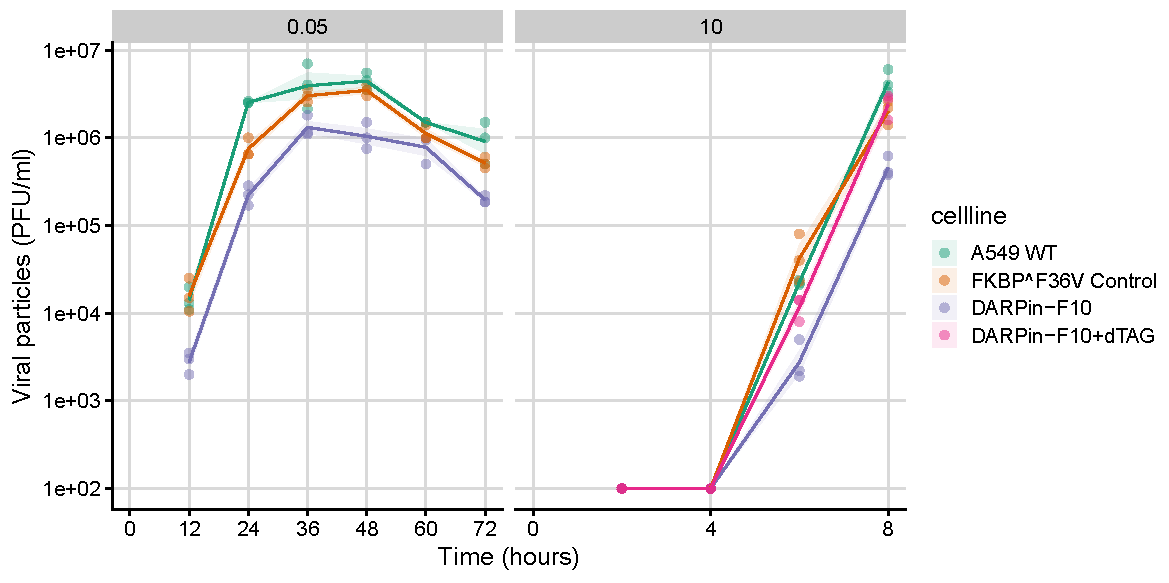
\includegraphics[width=0.95\textwidth, trim={0cm 0cm 0cm 0cm}, clip]{D_chapters/3_DARPinModels/DarpinVirusProduction.pdf}
\caption[Influence of varying individual initial protein abundances and reaction rate parameters on the capsid breakage probability]%
{A549 WT: wild type;\par
FKBP\textasciicircum F36V Control: cell line with a different mutation.\par
DARPin-F10: cells with a DARPin that binds HDAC6 ZnF;\par
DARPin-F10 + dTAG: cells in which DARPin F10 was degraded through dTAG before virus infection.}
\label{figure:darpinProductionExperimental}
\end{center}
\end{figure}

They showed that DARPin-F10 has a high specificity and affinity against HDAC6-ZnF \cite{DarpinData}. They were able to stably express and reversibly DARPin F10 in A549 cells. Using these new mutant cell lines they demonstrated that at multiplicity of infection (MOI) of 30 PFU/ml DARPin-F10 expression leads to the reduction in influenza viral uncoating (Figure \ref{figure:darpinUncoatingExperimental}), and at MOIs of 10 and 0.05 PFU/ml - to reduction virus production (Figure \ref{figure:darpinProductionExperimental}).

Knowing that DARPin-F10 binds to HDAC6-ZnF we can with reasonable confidence assume that during influenza uncoating it acts as a competitor against polyubiquitin chains. 

In this chapter, we use that assumption, and introduce DARPin-F10 to our HDAC6 complex formation models. We make predictions about DARPin-F10 active concentrations and dose-response behavior, and discuss the possibly of using these predictions to determine whether "Symmetric" or "Asymmetric" model best describes the biological system.